\subsection{Subsystem 1: Processing}

\subsubsection{Subsystem Diagrams}
\begin{figure}[h]
    \centering
    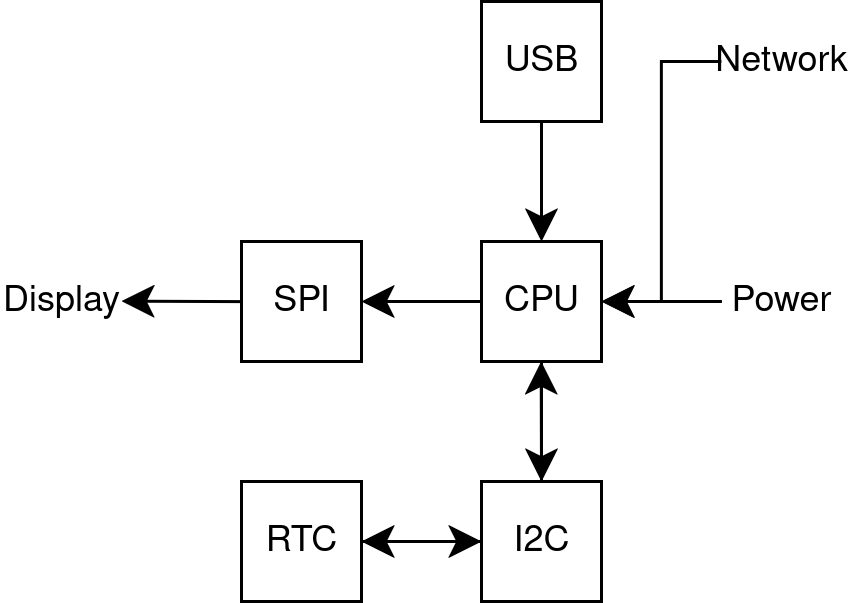
\includegraphics[width=12cm]{images/Processing_Subsystem_Block_Diagram.png} % Change the picture
    \caption{Subsystem Block Diagram}
\end{figure} % If your subsystem is more coding, change it to activity diagram

% Specifications
\subsubsection{Specifications}
\begin{enumerate}
    \item Support SPI clock $\geq$ 20 MHz
    \item SPI support up to 40 MHz, full-duplex, DMA capable
    \item Display update latency $\leq$ 16 ms
    \item Support configurable API refresh interval between 60 and 300 s
    \item API end-to-end fetch latency $\leq$ 2 s
    \item Clock drift $\leq \pm 1\frac{\text{sec}}{\text{day}}$
    \item Operating voltage: $3.3 \pm 0.1$ V
\end{enumerate}

% Subsystem Interactions
\subsubsection{Subsystem Interactions}
The core computer interfaces with
all other subsystems. The battery/power
management unit supplies it with power.
Running processes direct and receive
information from the network module.
It communicates with the digital dot matrix
display via SPI according to display
drivers on the controller.


% Core ECE
\subsubsection{Core ECE Design Tasks}
\begin{itemize}
    \item \textbf{ENGR 16100}: Teamwork \& project documentation.
    \item \textbf{CS 15900}: Fundamentals of programming.
    \item \textbf{ECE 36200}: PCB design and embedded software development.
\end{itemize}

% Schematics
\subsubsection{Schematics}
[Type here \textbf{DD2+}]
\begin{figure}[h]
    \centering
    
\includegraphics[width=16cm]{images/white.png} % Change the picture
    \caption{[Schematic Name]}
\end{figure} % If your subsystem is more coding, change it to psudo code

% Parts List
\subsubsection{Parts}
\begin{itemize}
    \item ESP32-S3
    \item DS3231
    \item PCB
\end{itemize}

% Algorithm
\subsubsection{Algorithm}
\begin{lstlisting}
    initialize clock, network, display, location

    always 
        wifi keep alive
        error handling
    
    every minute
        update display time

        make API call for flight data
        parse data

        if battery powered
            check battery voltage
            add battery to data

        add time, weather, flight info to data
        convert data to pixel buffer
        push pixel buffer to display
    
    every hour
        sync RTC with network time

        make API call for weather

\end{lstlisting}

% Theory of Operation
\subsubsection{Theory of Operation}
[Type here \textbf{DD2+}]

% Specification Measurement
\subsubsection{Specifications Measurement}
[\textbf{DD3+} Every specification here should match the specification above. ]
\begin{enumerate}
    \item {[Copy specification here. ]} \\
          {[Explain the specification here. Add photoes if necessary. ]}
\end{enumerate}

% Standards
\subsubsection{Standards}
\begin{itemize}
    \item \textbf{IPC-2221}: Governs PCB trace width, spacing, creepage/clearance, via rules, grounding, etc.
    \item \textbf{IPC-A-610}: Covers soldering quality and workmanship.
    \item \textbf{RFC 5905}: Protocol for syncing ESP time to internet.
\end{itemize}